\section{MMC}

\subsection{MMC steps during booting}

\begin{itemize}

\item configures CPU, UART
\item sets port directions
\item enables VCCINT PSU
\item enables P5V0 PSU (helper PSU)
\item enables Exar PSU. It boots from its own EEPROM
\item waits 200ms
\item configures SCANSTA chip in stitcher mode. If RTM is inserted, it enables its JTAG port
\item configures I2C switch base address
\item initializes default RTM power state to off
\item initializes Ethernet PHY chip in RGMII mode using pin strap.
\item waits 200ms
\item initializes I2C controller and chain (switch)
\item configures Si5324
\item checks if RTM is inserted, if yes, then enables its power, waits 200ms and initializes RTM power supply via I2C. It also configures Si5324 on RTM
\item runs task.\\

The task performs following functions:

\item blinks front panel LEDs alternately
\item checks if FPGA is configured. If not, it keeps Ethernet PHY in reset state. Once FPGA gets configured, it initializes the PHY.
\item checks if RTM is unplugged. If not, it switches the power off to make sure it is off during hotplug.
\end{itemize}

\subsection{Bootstraping}

The MMC can be upgraded by USB cable and NXP programmer(can be used other programmer but make sure that header shorts pins 3, 5, 9) using  \href{http://www.flashmagictool.com/}{Flashmagic} or any other software which can talk with NXP bootloader. The source code is written in C and can be found on github.\\ 
\textbf{Source code:} \href{https://github.com/m-labs/sinara/tree/master/SAYMA\_firmware}{https://github.com/m-labs/sinara/tree/master/SAYMA\_firmware}.\\
\textbf{pre-compiled binary:} \href{https://github.com/m-labs/mmc-firmware/releases}{https://github.com/m-labs/mmc-firmware/releases}\\

To compile binaries \href{https://www.nxp.com/products/processors-and-microcontrollers/arm-based-processors-and-mcus/lpc-cortex-m-mcus/lpc1100-cortex-m0-plus-m0/lpcxpresso-ide-v8.2.2:LPCXPRESSO?tab=Design_Tools_Tab}{LPCXpresso} is needed.

\subsection{Functionality}

\todo[inline]{needed?}

\subsection{Exar debugging}
 
In case of chip failure, i.g.overvoltage, overcurrent, etc., there is possibility  to check chip status via UART. In this case in UART console, Exar register readout can be done by typing 'P' character.\\

	\begin{figure}[htbp!]
		\centering
		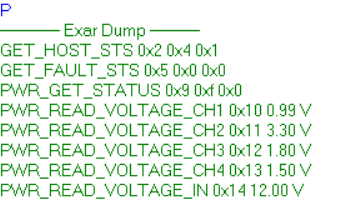
\includegraphics[scale=0.6]{img/exarreg.png}\\
		\caption{Exar register } 
	\end{figure}	
\clearpage
\subsection{PHY debugging}

In case of chip failure, there is possibility to check chip status via UART. In this case in UART console, Ethernet PHY content can be read by typing 'E' character

	\begin{figure}[htbp!]
		\centering
		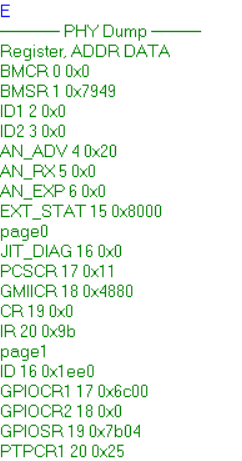
\includegraphics[scale=0.6]{img/phyreg.png}\\
		\caption{Ethernet PHY register } 
	\end{figure}

\subsection{RGMII Ethernet }

\todo[inline]{TBD. Not sure what should it contain.}

\subsection{OpenMMC}

\textbf{OpenMMC Project:}\href{https://github.com/lnls-dig/openMMC}{https://github.com/lnls-dig/openMMC}

\todo[inline]{TBD}
